\documentclass{article}    

\usepackage{graphicx}

\begin{document}

% ------------------------------------------ figure 2

\begin{figure}[!ht] \centering
  \begin{tabular}{ccc}
    
\includegraphics[height=0.16\textheight]{Electrode.eps} &
    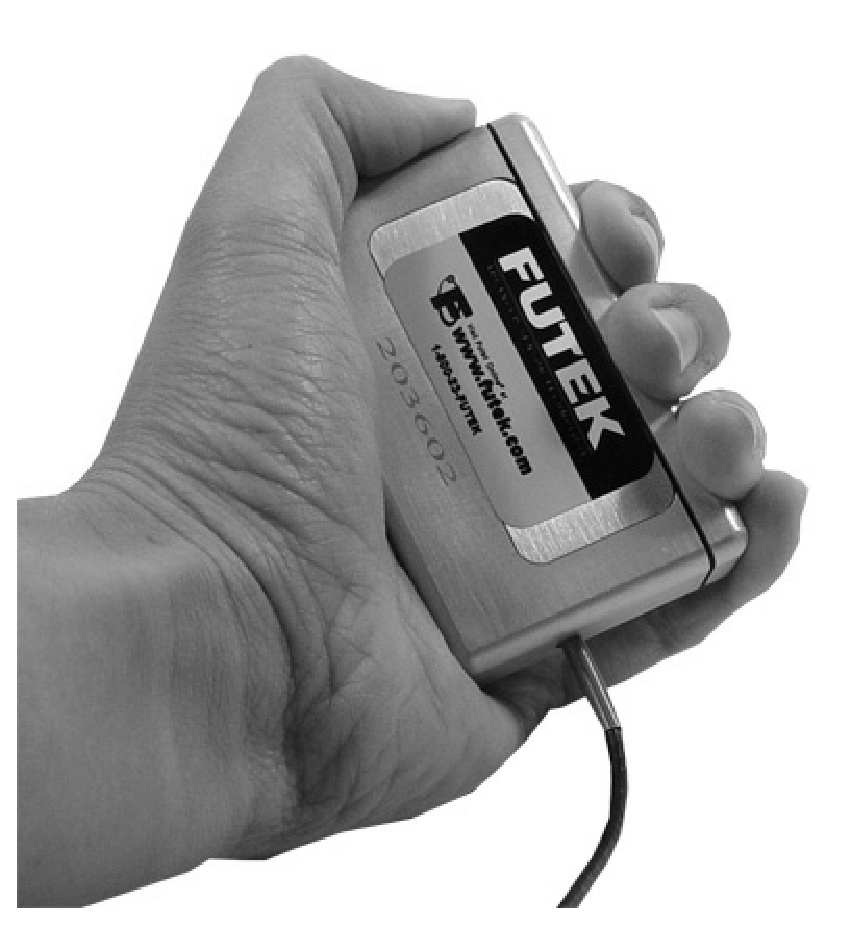
\includegraphics[height=0.16\textheight]{Hand_Gripper.eps} &
    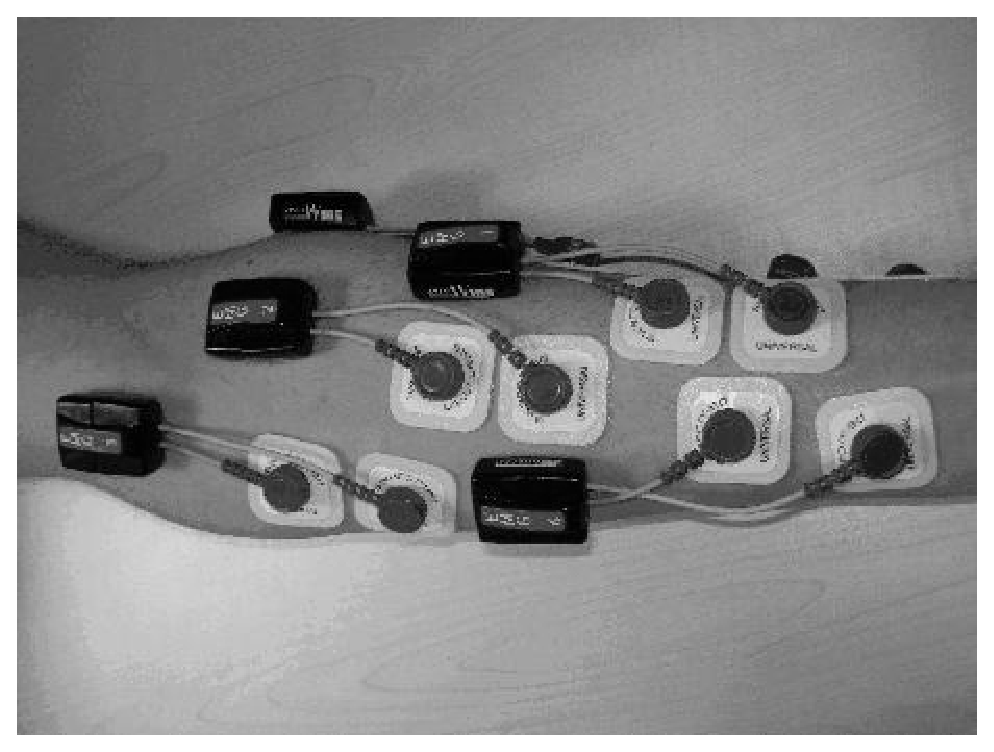
\includegraphics[height=0.16\textheight]{El_Arrangement.eps} \\
    $(a)$ & $(b)$ & $(c)$ \\
  \end{tabular}
%  \caption{The experimental setup (\textit{subject side}): $(a)$ an EMG
%    wireless electrode; $(b)$ the FUTEK force sensor; $(c)$ the typical
%    placement of the EMG electrodes on a subject's forearm (ventral side).}
%  \label{fig:SubjSetup}
\end{figure}

\end{document}
